%追加すべき事項
% - 実験結果の画像の添付
% - DDSP解説?
% - ? Adamの説明
\appendix

\chapter{Adam}
\label{app:Adam}

Adamは勾配降下法の中で最も用いられるアルゴリズムであり、\prettyref{alg:Adam}に示す手順にしたがってパラメータの更新を行う。また、Adamについては~\cite{Adam}に詳しい。

\begin{algorithm}[b]
\label{alg:Adam}
    \DontPrintSemicolon
    \SetKwInOut{KwHyParam}{HyperParameter}
    \SetKwInOut{KwParam}{Parameter}
    \SetKwInOut{KwObFunc}{Objective~Function~}
    \SetKwProg{Init}{Initialization}{:}{end}
    \SetKwProg{Proc}{Procedure}{:}{end}
    \KwHyParam{$\beta_1,\beta_2\in \interval[open left]{0}{1},\eta,\epsilon$}
    \KwObFunc{$f$}
    \KwParam{$\theta$}
    \BlankLine
    \Init{}{
        $t \leftarrow 0$ \tcc*{Initialize~timestep}
        $\theta \leftarrow \theta_0$ \tcc*{Initialize~Parameter}
        $m_1 \leftarrow 0$ \tcc*{Initialize~$1^{st}$~moment}
        $m_2 \leftarrow 0$ \tcc*{Initialize~$2^{nd}$~moment}
    }
    \BlankLine
    \Proc{}{
        \While{$\theta$ not converged}{
            $t \leftarrow t+1$ \tcc*{Update~timestep}
            $g \leftarrow \nabla _{\theta} f(\theta)$ \tcc*{Compute~gradient~of~$f(\theta)$}
            $m_1 \leftarrow \beta_1 \cdot m_1+(1-\beta_1) \cdot g$ \tcc*{Update~biased~$1^{st}$~moment}
            $m_2 \leftarrow \beta_2 \cdot m_2+(1-\beta_2) \cdot (g \odot g)$ \tcc*{Update~biased~$2^{nd}$~moment}
            $\hat{m_1} \leftarrow m_1/(1-\beta_1^t)$ \tcc*{Compute~bias-corrected~$1^{st}$~moment}
            $\hat{m_2} \leftarrow m_2/(1-\beta_2^t)$ \tcc*{Compute~bias-corrected~$2^{nd}$~moment}
            $\theta \leftarrow \theta - \eta \cdot \hat{m_1}/(\sqrt{\hat{m_2}}+\epsilon)$ \tcc*{Update~Parameter}
        }
        \Return{$\theta$}
    }
    \BlankLine
\caption{Adamの疑似コード}
\end{algorithm}

\chapter{学習時のパラメータ}
\label{app:params}

提案モデルの学習時のパラメータの値を\prettyref{tab:params1}に示す。また、\prettyref{tab:params2}は\prettyref{alg:Adam}に示すハイパーパラメータの値である。

\begin{table}[h]
\centering
\begin{minipage}{0.49\columnwidth}
    \centering
        \begin{tabular}{lr}\toprule
            パラメータ & 値 \\ \midrule
            バッチサイズ & 1 \\ 
            エポック数 & 1000 \\ \bottomrule
        \end{tabular}
    \caption{}
    \label{tab:params1}
\end{minipage}
\begin{minipage}{0.49\columnwidth}
    \centering
        \begin{tabular}{lr}\toprule
            パラメータ & 値 \\ \midrule
            $\beta_1$ & 0.5 \\
            $\beta_2$ & 0.999 \\
            $\eta$ & 0.0002 \\ 
            $\epsilon$ & $10^{-8}$ \\ \bottomrule
        \end{tabular}
    \caption{}
    \label{tab:params2}
\end{minipage}
\end{table}

\chapter{データセットの分割}
\label{app:split}

22音ずつの4つのサブセットにデータセットを分割した~(\prettyref{fig:data_div})~。また、データセットの4分割は、88音をシャッフルして配列に格納した後に22音ずつ順に選ぶことで実装した。

\begin{figure}[h]
\centering
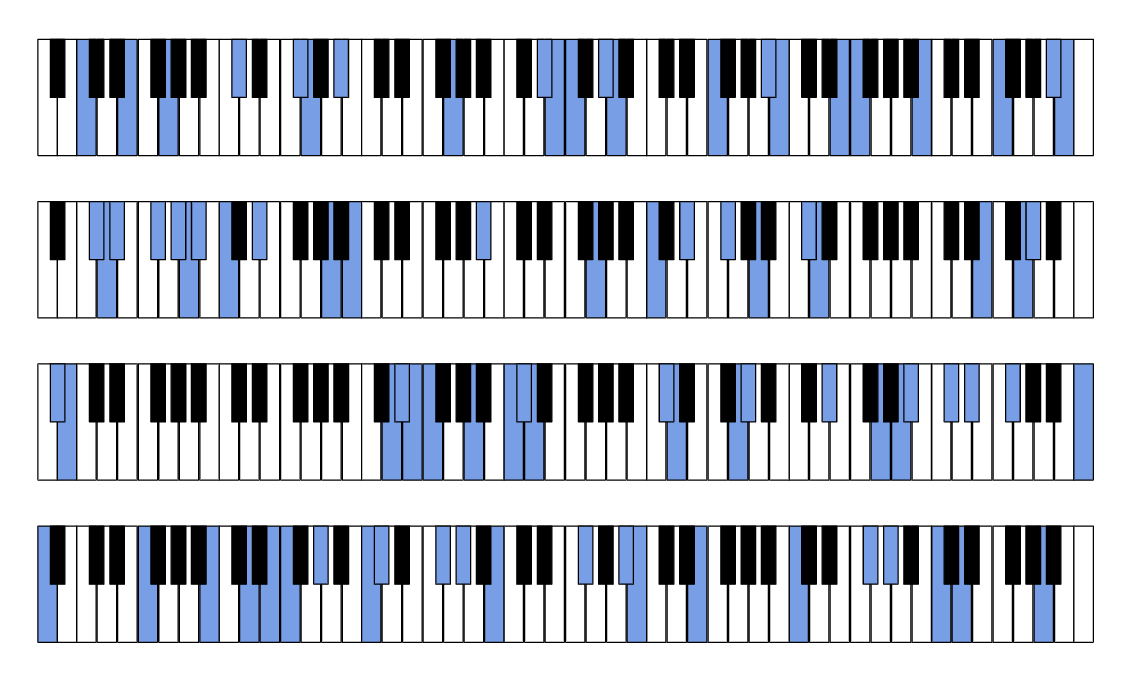
\includegraphics[width=\columnwidth]{figure/data_div.png}
\caption{データセットのサブセット}
\label{fig:data_div}
\end{figure}

\chapter{DDSP}
\label{app:DDSP}

\chapter{実験結果}
\label{app:result}

\prettyref{sec:result}に載せることのできなかった波形の図を本章に載せる

\section{提案モデルの表現力の評価実験}

提案モデルの評価実験を行ったところ、88音のうち87音については変換先のギターの音を表現できていると判断することができた。


\section{提案モデルの汎化能力の評価実験}